\section{}
A 20-mm-thick steel bar with a slot (25-mm radii at ends) is subjected to an axial load $P$, as shown in Figure \ref{fig:Q4ProblemDiagram}.
What is the maximum stress for $P = \qty{180}{\kilo\newton}$? Use Fig. D.8B to estimate the value of $K$.

\begin{figure}[h]
    \centering
    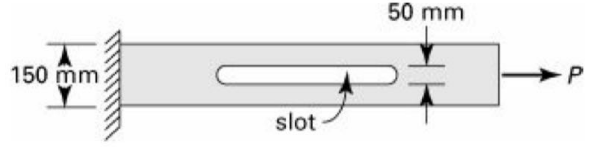
\includegraphics[width=0.5\linewidth]{Questions/Figures/Q5ProblemDiagram.png}
    \caption{Problem diagram for Question 5.}
    \label{fig:Q5}
\end{figure}

Finding the stress at the slot ends (circular hole), $d = \qty{50}{\milli\meter}$, $D = \qty{150}{\milli\meter}$, $t = \qty{20}{\milli\meter}$.
Then, $d/D = 1/3$ which, from Fig. D.8B, $K = 2.3$.
\begin{figure}[h]
    \centering
    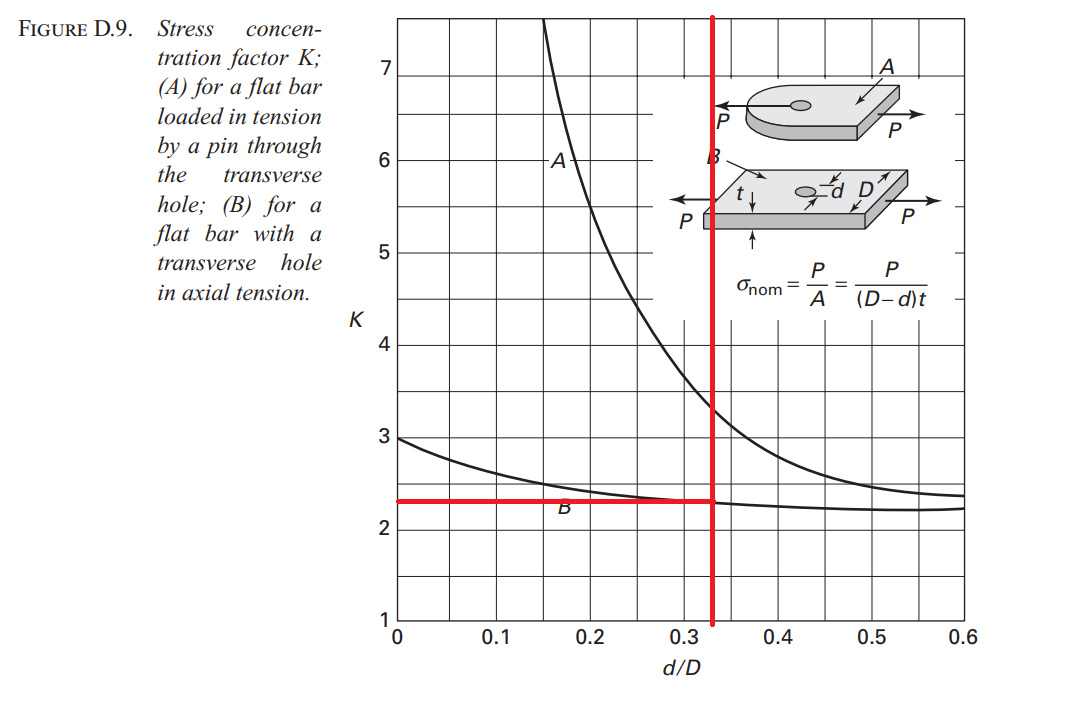
\includegraphics[width=0.5\linewidth]{Questions/Figures/Q5Chart.png}
    \caption{Chart for Question 5.}
    \label{fig:Q5Chart}
\end{figure}
Finding the nominal stress using
\begin{align*}
    \sigma_{\text{nom}} &= \frac{P}{(D-d)t} \\
    &= \frac{180\times 10^3}{(150-50)(20)\times 10^{-6}} \\
    &=\qty{90}{\mega\pascal}
\end{align*}
Finding the maximum stress using $K$,
\begin{align*}
    \sigma_{\text{max}} &= K \sigma_{\text{nom}} \\
    &= (2.3)(90) \\
    &= \boxed{\qty{207}{\mega\pascal}}
\end{align*}